\documentclass[fleqn]{jbook}
\usepackage{physpub}

\newcommand{\W}{\vec{\mathbf{W}}} %Wベクトル
\newcommand{\vu}{\vec{\mathbf{u}}} %uベクトル
\newcommand{\vv}{\vec{\mathbf{v}}} %vベクトル
\newcommand{\rd}{\partial} %偏微分

\begin{document}

\begin{question}{問題4}{諏訪 雄大}
宇宙探査機は燃料の不足を補うため、しばしばスイングバイという航法で加速を行うことがある。(例えばアポロ13号は月の重力を、火星探査機のぞみは地球の重力を使って加速した。)中心力場の力学からこの原理について考える。
\begin{enumerate}
\item 2次元の極座標系$(r,\phi)$を用いて中心力ポテンシャル$U(r)$中を運動する質量$m$の質点のLagrangianを書き、Euler-Lagrangeの方程式を用いて角運動量の保存則を導け。
\item 図1のように質量$m$の探査機が質量$M$の惑星に対して距離$b$の漸近線$SS'$に沿って無限遠方から速さ$v$で進入し、漸近線$TT'$に沿って出てゆくものとする。ただし、$M\gg m$の関係があり、惑星は静止しているとみなしてよい。惑星の位置を原点とし、探査機の座標を$(r,\phi)$とするとき次式が成り立つことを示せ。
	\begin{eqnarray}\ilabel{4_1}
	\dot\phi=\frac{vb}{r^2}
	\end{eqnarray}

   	\begin{figure}[htbp]
	    \begin{center}
		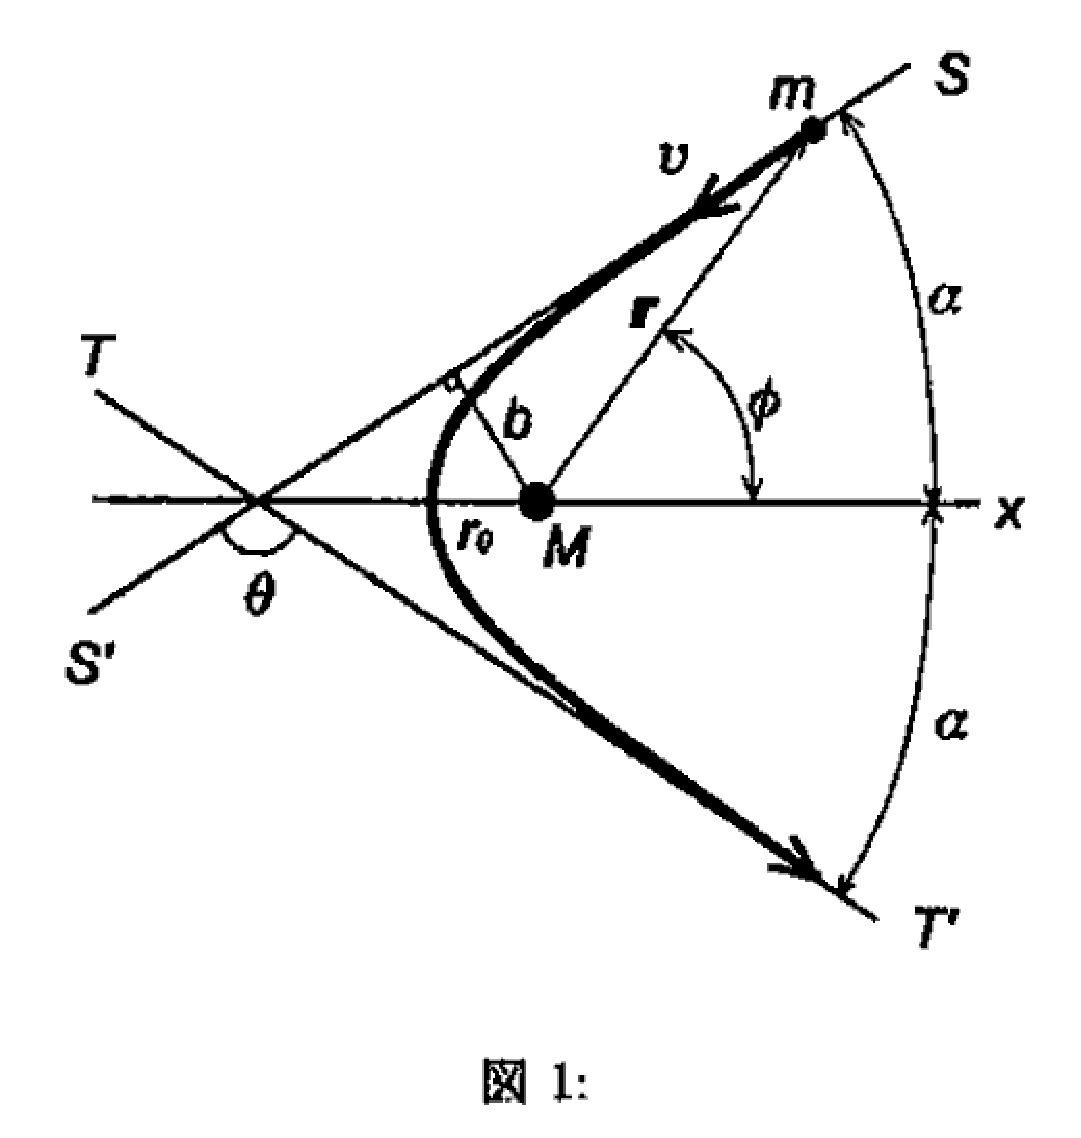
\includegraphics[width=95mm]{2003phy4-1.eps}
	    \end{center}
	\end{figure}

\item 探査機が惑星に最も近づいた時の惑星までの距離$r_0$を、$v,b,M$と重力定数$G$を用いて表せ。ただし、ポテンシャル$U(r)は、U(r)=-\frac{GMm}{r}$と表される。
\item 探査機の$(x,y)$座標系における速度を$(v_x,v_y)$とおくと、$v_xと\phi$の間に次の微分方程式が成立することを示せ。ただし、式(\iref{4_1})を用いてよい。
	\begin{eqnarray}\ilabel{4_2}
	dv_x=-\frac{GM}{vb}\cos\phi d\phi
	\end{eqnarray}
\item 入射前後における角度変化$\theta$が$\tan\frac{\theta}{2}=\frac{GM}{v^2b}$で表されることを示せ。ただし、式(\iref{4_2})を用いてよい。
	\item 図2のように惑星が速度ベクトル$\W$で太陽に対して運動していたところへ探査機がやってきた。探査機の太陽に対する相対速度ベクトルが入射前は$\vv$、出射後は$\vu$であったとして、惑星の運動量の変化を無視せずに、入射前後における探査機のエネルギー変化、$\frac{1}{2}m|\vu|^2-\frac{1}{2}|\vv|^2$を求めよ。ただし、惑星の引力圏では、太陽からの引力は無視できるものとする。
	\item 上の結果から探査機の加速が可能なことを示せ。また、増加した探査機のエネルギーはどこから来たか答えよ。

      \begin{figure}[htbp]
	  \begin{center}	 
	      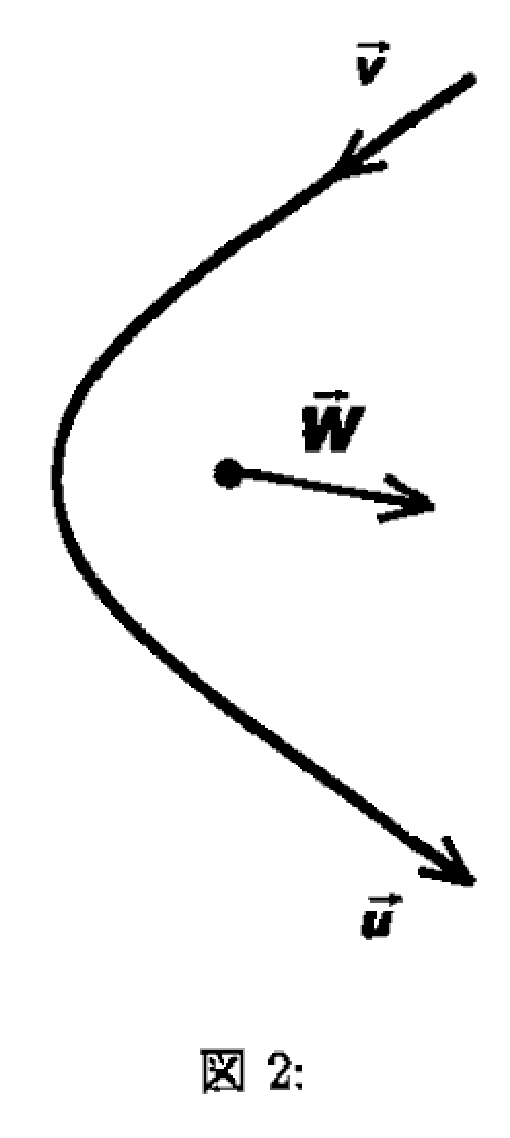
\includegraphics[width=40mm]{2003phy4-2.eps}
	  \end{center}
      \end{figure}

\end{enumerate}
\end{question}

\begin{answer}{問題4}{諏訪 雄大}
\begin{enumerate}
\item 粒子のLagrangianは、
	\begin{eqnarray*}
	L&=&\frac{p^2}{2m}-U(r)\\
	&=&\frac{1}{2}m(\dot r^2+r^2\dot\phi^2)-U(r)
	\end{eqnarray*}
	と書ける。これを以下のEuler-Lagrange方程式に代入すると、
	\[
	\frac{\rd L}{\rd\phi}-\frac{d}{dt}\frac{\rd L}{\rd\dot\phi}=0
	\]
	\[
	∴\ \frac{d}{dt}(mr^2\dot\phi)=0
	\]
	したがって、角運動量$mr^2\dot\phi$が保存されることが示された。
\item 無限遠での探査機の角運動量は$mvb$であるから、1で得られた角運動量の保存則より、
	\[
	mr^2\dot\phi=mvb
	\]
	\[
	∴\ \dot\phi=\frac{vb}{r^2}
	\]
\item 1のLagrangianを以下のEuler-Lagrange方程式に代入すると、$\dot\phi=\frac{vb}{r^2}$を用いて、
	\begin{eqnarray*}
	\frac{\rd L}{\rd r}-\frac{d}{dt}\frac{\rd L}{\rd\dot r}&=&0\\
	mr\dot\phi^2-\frac{\rd U}{\rd r}-\frac{d}{dt}(m\dot r)&=&0\\
	m\frac{v^2b^2}{r^3}-\frac{GMm}{r^2}-m\ddot r&=&0
	\end{eqnarray*}
	という式が成り立つ。これは下のように書き換えられる。
	\begin{eqnarray*}
	m\ddot r&=&m\frac{v^2b^2}{r^3}-\frac{GMm}{r^2}\\
	&=&-\frac{d}{dr}\bigg(\frac{mv^2b^2}{2r^2}-\frac{GMm}{r}\bigg)
	\end{eqnarray*}
	ここで、上の式の右辺を$-\frac{d}{dr}\tilde U(r)$とすれば、$\tilde U(r)$は有効ポテンシャルとなる。
	無限遠で探査機のもつエネルギーは、$\frac{1}{2}mv^2$であるから、
	\[
	\frac{1}{2}mv^2=\frac{mv^2b^2}{2r^2}-\frac{GMm}{r}
	\]
	の解が$r_0$となる。これを解くと、
	\[
	r_0=\frac{-GM+\sqrt{G^2M^2+v^4b^2}}{v^2}
	\]
	となる。
\item $x$方向の力について考える。\\
	重力の方向の$x$方向の力は、
	\[
	-\frac{d}{dr}\bigg(-\frac{GMm}{r}\bigg)\cos\phi=-\frac{GMm}{r^2}\cos\phi
	\]
	となるから、以下の式が成り立つ。
	\[
	m\ddot x=-\frac{GMm}{r^2}\cos\phi
	\]
	ここで、$\dot x=v_x$と書くと、
	\[
	m\frac{dv_x}{dt}=-\frac{GMm}{r^2}\cos\phi
	\]
	両辺に$\frac{dt}{d\phi}=\frac{1}{\dot\phi}$をかけると、
	\begin{eqnarray*}
	\frac{dv_x}{d\phi}&=&-\frac{GM}{r^2\dot\phi}\cos\phi\\
	&=&-\frac{GM}{vb}\cos\phi
	\end{eqnarray*}
	したがって、
	\[
	dv_x=-\frac{GM}{vb}\cos\phi d\phi
	\]
	が示された。
\item (\iref{4_2})の両辺を積分すると、
	\[
	v_x\bigg|_{入射前}^{出射後}=-\frac{GM}{vb}\sin\phi\bigg|_{入射前}^{出射後}
	\]
	ここで、左辺の変化について考えると、$2v\sin\frac{\theta}{2}$となる。また、右辺は入射前の無限遠で$\phi\to \frac{\pi}{2}-\frac{\theta}{2}$、出射後の無限遠で$\phi\to -\frac{\pi}{2}+\frac{\theta}{2}$となることより、以下の式が成り立つ。
	\begin{eqnarray*}
	2v\sin\frac{\theta}{2}&=&\frac{GM}{vb}\{\sin(\frac{\pi}{2}-\frac{\theta}{2})-\sin(-\frac{\pi}{2}+\frac{\theta}{2})\}\\
	&=&\frac{GM}{vb}2\cos\frac{\theta}{2}
	\end{eqnarray*}
	これをまとめると、
	\[
	\tan\frac{\theta}{2}=\frac{GM}{v^2b}
	\]
	が示される。
	\item 前提として、惑星の運動量は変化は考えるが、速度単体の変化は微小なため、無視するものとする。
	
	このとき、惑星の静止系で見ると、探査機は双曲線軌道を描くので、入射速度と出射速度が等しくなる。
	これを式で書くと、
	\[
	|\vv-\W|=|\vu-\W|
	\]
	両辺を2乗してまとめると、
	\[
	|\vu|^2-|\vv|^2=2(\vu-\vv)・\W
	\]
	したがって、入射前後における探査機のエネルギー変化は、
	\[
	\frac{1}{2}m|\vu|^2-\frac{1}{2}m|\vv|^2=m(\vu-\vv)・\W
	\]
	と得られる。
	\item 太陽の静止系で見た探査機の速度ベクトルの変化($\vu-\vv$)は、惑星の静止系で見た速度ベクトルの変化($(\vu-\W)-(\vv-\W)$)に等しい。このとき、入射速度ベクトルによって、$\vu-\vv$の方向は変わるが、それを上手く選んでやれば、$(\vu-\vv)・\W>0$とすることができる。この条件下で、6.で求めた入射前後における探査機のエネルギー変化が正となるので、探査機は加速可能なのである。
	
	次に、そのエネルギー変化量の起源は、惑星の公転エネルギーである。以下でそれを示す。
	
	まず、運動量保存の法則より、探査機出射後の惑星の運動量を$\W'$とすると、
	\[
	m\vv+M\W=m\vu+M\W'
	\]
	と書ける。したがって、
	\[
	\W'=\W+\frac{m}{M}(\vv-\vu)
	\]
	これを用いて、惑星の運動エネルギーの変化量$\frac{1}{2}M(|\W'|^2-|\W|^2)$を求めると、
	\[
	\frac{1}{2}M(|\W'|^2-|\W|^2)=-m(\vu-\vv)・\W
	\]
	と得られる。ちなみに、この計算において、$\big(\frac{m}{M}\big)^2$の項は微小であるので無視した。これは、6.で求めた探査機の運動エネルギー変化の符号を変えたものに等しい。つまり、惑星が失ったエネルギーを探査機が受け取ったのである。したがって、探査機得たエネルギーの源が惑星の公転の運動エネルギーであることが示された。
\end{enumerate}
\end{answer}


\end{document}
